%!TEX root = ../main.tex

\section{CRF Learning for OCR [30 pts] (Yifeng)}

\textbf{Note: Please submit all your answer (including derivations, calculated values, figures) to this problem in the pdf file, the executable code and provided dataset in the *.zip file.}

\subsection{Introduction}
In this problem, you will implement your own code to learn the parameters of a conditional random field (CRF) for optical character recognition (OCR).

In the CRF model, there are two kinds of variables: the hidden variables that we want to model and those that are always observed. In the case of OCR, we want to model the character assignments (such as ‘a’ or ‘c’), and we always observe the character images, which are arrays of pixel values. Typically, the unobserved variables are denoted by $Y$ and the observed variables are denoted by $X$. The CRF seeks to model $P(Y |X)$, the conditional distribution over character assignments given the observed images. We will be working with the OCR model that includes only the singleton and pairwise factors (as we will explain in detail below). The structure of the model is shown below:

\begin{figure}[h]
	\centering
	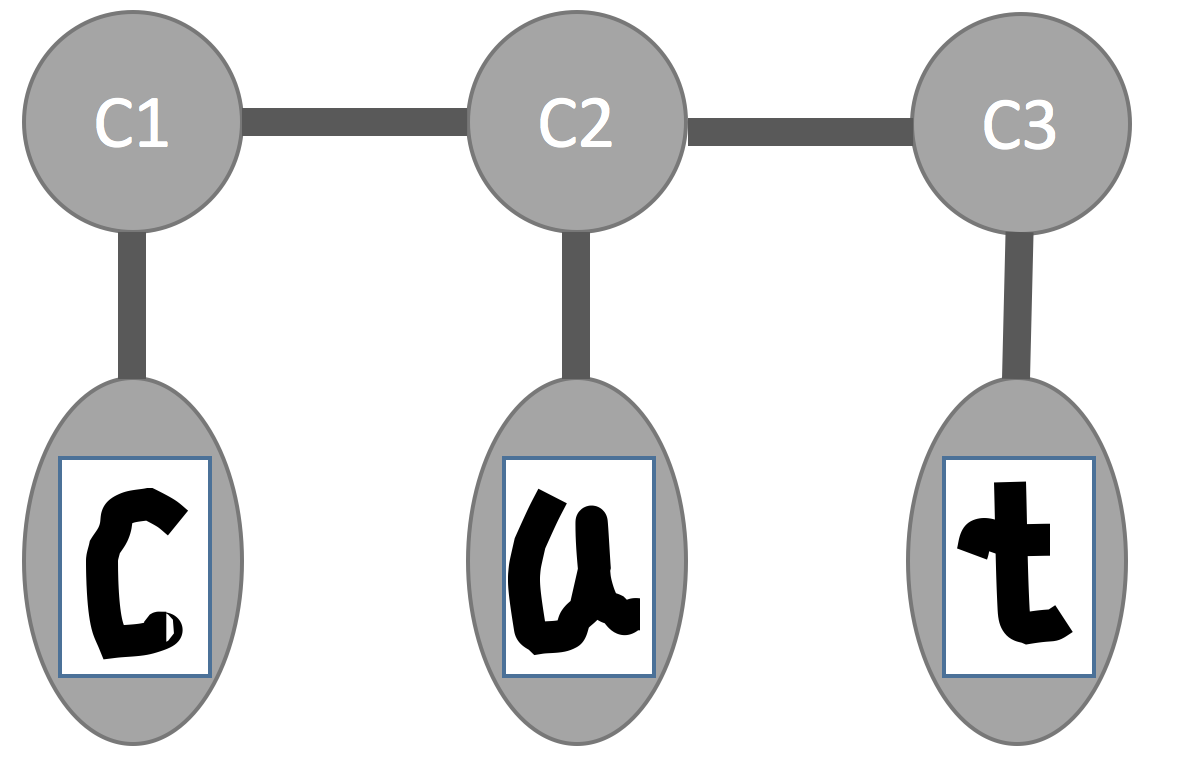
\includegraphics[width = 0.3\linewidth]{figures/figCRF1.png}
	\caption{CRF with singleton and pairwise factors.}
\label{fig:crf}
\end{figure}

As you can see, our CRF for OCR is a specific case of the general CRF mentioned in class. Specifically, you will build the model around log-linear features. A feature is just a function $f_i (D_i)$: $Val(D_i) \rightarrow \mathbb{R}$, where $D_i$ is the set of variables in the scope of the $i$-th feature. Here, all features are binary indicator features (taking on a value of either 0 or 1). Each feature has an associated weight $\theta_i$. Given the features $\{f_i\}_{i=1}^k$ and the weights $\{ \theta_i  \}_{i = 1}^k$, the distribution is defined as:
\begin{align}
P(Y | X; \theta) = \frac{1}{Z_X (\theta)}  \exp \{  \sum_{i=1}^{k} \theta_i f_i (D_i)  \}.
\end{align}
The term $Z_X (\theta)$ is the partition function:
\begin{align}
Z_X (\theta) = \sum_Y \exp \{ \sum_{i=1}^k \theta_i f_i ( D_i )  \}.
\end{align}

In our CRF, we have three types of features:
\begin{itemize}
	\item $f_{i,c}^C ( Y_i )$, which operates on single characters / hidden states (an indicator for $Y = c$).
	
	\item $f_{i,j,c,d}^I ( Y_i, X_{ij})$,which operates on a single character / hidden state and an image pixel	associated with that state (an indicator for $Y_i = c, X_{ij} = d$). These are collectively used to encode the individual probability that $Y_i = c$ given $X_i$.
	
	
	\item $f_{i,c,d}^P (Y_i, Y_{i+1})$which operates on a pair of adjacent characters / hidden states (an indicator for $Y_i = c, Y_{i+1}  = d$).
	
\end{itemize}


\subsection{Gradient of Negative Log-likelihood  [5pts]}

Our goal is to maximize the log-likelihood of the parameters given the data. Thus the cost / loss we minimize is simply the negative log-likelihood, together with a $L_2$-regularization penalty on the parameter values to prevent overfitting. The function we seek to minimize is:
\begin{align}
\text{nll} (X, Y, \theta) = \log(Z_X(\theta))  - \sum_{i =1}^{k} \theta_i f_i (Y, X) + \frac{\lambda}{2} \sum_{i = 1}^{k} \theta_i^2.
\end{align}

\textbf{Question: }Please prove that partial derivatives for this function have an elegant form:
\begin{align}
\frac{\partial }{\partial \theta_i} \text{nll} (X, Y, \theta) = E_{\theta} [ f_i ] - E_D [ f_i] + \lambda \theta_i,
\end{align}
where
\begin{align}
E_{\theta} [f_i] &= \sum_{Y'} P( Y' | X) f_i (Y', X), \\
E_D [ f_i ] &= f_i (Y, X).
\end{align}
We drop the $\theta$ from $P(Y' | X)$ for convenience.


\subsection{Shared Parameters [2pts]}

There is one more detail to take care of: shared parameters across multiple features. Parameter sharing is a form of templating used to reduce the total number of parameters we need to learn. Let $\{f^{(i)}  \}$ be the set of features that share parameter $\theta_i$. 

\textbf{Question: }Give a brief explanation that we can expend the equations (3, 4) above as:
\begin{align}
\text{nll} (X, Y, \theta) = \log ( Z_X (\theta) ) - \sum_{i=1}^{k} \theta_i (  \sum_{f_j \in \{ f^{(i)} \} }  f_j (Y, X ) ) + \frac{\lambda}{2} \sum_{i = 1}^k \theta_i^2.
\end{align}
\begin{align}
\frac{\partial }{\partial \theta_i} \text{nll} (X, Y, \theta) =  \sum_{ f_j \in \{ f^{(i)}   \}   } E_{\theta} [ f_j ] - \sum_{  f_j \in \{ f^{(i)}  \}  }  E_D [ f_i] + \lambda \theta_i.
\end{align}
Note that in this case, $\theta_i$ is not necessarily related to $f_i$ any longer. Instead, $\theta_i$ is associated with a set of features $\{ f^{  (i)  }  \}$. $k$ is the total number of parameters of $\theta_i$, and not necessarily the total number of features $f_j$. The parameters that we use in the CRF are:
\begin{itemize}
\item $\theta_c^C$, shared by $ \{  f_{i,c}^C (  Y_i  )    \}_i   $.

\item $\theta_{c,d}^I$, shared by $ \{   f_{i,j,c,d}^I  (  Y_{i}, X_{ij}   )          \}_{i,j}       $.


\item $\theta_{c,d}^P$, shared by $ \{   f_{i,c,d}^P (Y_i, Y_{i+1})      \}_i  $.
\end{itemize}
Essentially, this parameter tying scheme ties parameters across different locations together; that is, a character at the start of the word shares the same parameters as a character at the end of the word.


\subsection{InstanceNegLogLikelihood Implementation [18pts]}

Given this discussion, we can now state your mission: for a given data instance $(X,Y)$ and a parameter setting $\theta$, you must compute the cost function (regularized negative log-likelihood) and the gradient of parameters with respect to that cost. Doing so involves six terms (ignoring the issue of shared parameters in these):

\begin{itemize}
\item The log partition function: $\log ( Z_X (\theta) )$

\item The weighted feature counts: $\theta_i f_i ( Y, X )$

\item The regularization cost: $ \frac{\lambda}{2} \sum_{i=1}^k \theta_i^2$

\item The model expected feature counts: $\sum_{Y'}  P(Y' | X) f_i (Y', X) $

\item The data feature counts $f_i (Y, X)$

\item The regularization gradient term: $\lambda \theta_i$.

\end{itemize}

In this problem, you are provided with a single instance and related parameters in \verb|q2instance.mat| to help you implement your \verb|InstanceNegLogLikelihood| function, which should return the negative log-likelihood and gradient of the parameters. First, we should clarify what exactly we mean by a data “instance.” The input to \verb|InstanceNegLogLikelihood| function includes $X$ and $Y$ which together form a single instance $(X,Y)$. This instance corresponds to one
word, that is, a sequence of characters.

Thus, the variable $Y$ is a vector of character values. For example, $Y = (3, 1, 20)$ means that this instance contains the word “cat.” The variable $X$ is a matrix where the $i$-th row contains the pixel values for the ith character in the example. Each row has 32 values, since the images are 8x4 pixels. The feature sharing described above comes into play due to the fact that our data instances are not single images (as they were in the first part of the assignment) but instead sequences of images that we want to consider together.


\subsubsection*{(a) Number of Parameters [6pts] }

\textbf{Question:} Since we have a sequence of $Y$ with length 3, where each position has 26 hidden states; and each image has 32 binary positions. Considering the shared parameters across multiple features, show that $\theta$ has length of $2366$, i.e., clarify how many specific parameters in three different cases: $\theta_c^C, \theta_{c,d}^I, \theta_{c,d}^P$.

%26 + 26*26 + 26*(32*2) 
%each pixel has two states


\subsubsection*{(b) Implementation of InstanceNegLogLikelihood [12pts]}

Please implement your \verb|InstanceNegLogLikelihood| function:

\verb|[nll, grad] = InstanceNegLogLikelihood(X, y, theta, params)|.

\textbf{Question:} You are required to provide the following values in your pdf report:
\begin{itemize}
\item  \verb|sampleNLL|:  $\log ( Z_X (\theta) ) - \sum_{i=1}^{k} \theta_i (  \sum_{f_j \in \{ f^{(i)} \} }  f_j (Y, x ) ) + \frac{\lambda}{2} \sum_{i = 1}^k \theta_i^2$,

\item  \verb|sampleGrad(1:5)|: $\sum_{ f_j \in \{ f^{(i)}   \}   } E_{\theta} [ f_j ] - \sum_{  f_j \in \{ f^{(i)}  \}  }  E_D [ f_i] + \lambda \theta_i$,
\end{itemize}
where
\verb|[sampleNLL, sampleGrad] = InstanceNegLogLikelihood(sampleX, sampleY, sampleModelParams)|, and \verb|sampleX|, \verb|sampleY|, \verb|sampleTheta|, \verb|sampleModelParams| from \verb|q2instance.mat|:
Feel free to use any programming language you want and any resources from the Internet as soon as you acknowledge them properly.

% sampleNLL: 9.7743
% sampleGrad: [-0.8846         0   -0.9231    0.0385   -0.9231]



\subsection{Stochastic Gradient Descent [5pts]}

In this question, we want to train the CRF using stochastic gradient descent with vanishing step size.

In \verb|q2dataset.mat|, we provide \verb|trainData| and \verb|testData|. Each is a struct array with $X$ and $y$ fields. In both, each $(X, y)$ pair is the input the \verb|InstanceNegLogLikelihood|: $X$ gives the observations and $y$ gives the labels. You can directly use \verb|sampleModelParams| from \verb|q2instance.mat| as hyperparameters for training, and use \verb|sampleTheta| from \verb|q2instance.mat| for initialization of parameters.

\textbf{Question:} Train the model using stochastic gradient descent, plot the test loss versus training steps evaluated on the first 10 samples in the \verb|testData|. We only require you to train the model for one epoch (i.e., 220 steps in total), since the training is time consuming. We recommend using the learning rate of $\alpha_k = \frac{1}{1 + 0.05k}$, where $k$ is the number of steps.



